\documentclass[a4paper,10pt]{article}
\usepackage{a4wide}
\usepackage{listings}
\usepackage{mathtools}
\usepackage[english]{babel}
\usepackage{graphicx}
\begin{document}
\section*{Authors, date, assignment}
Authors : Dan Iatco (s2535130) \& Levente Sandor (s2552310)\\
Group: CS 1.Ib.1\\
Date:  13 December 2013\\
Day, Time of the Lab session: Thursday 28 November 2013, 15:00-17:00\\
Autonomous Systems lab 3 "Genetic Algorithms"\\

\section*{Exercise 1}

\section*{Exercise 2}
Eaters are primitive organisms which have a genetic code, DNA. At the start of their existance in the simulated world,
their DNA contain very few information about the world. They do not have any experience, and their movement is chaotic,
one cannot observe a low for their trajectory. As the time pass, the eaters evolve, and after 100 one can already observe
regularity in their movement, and also the numbers of plants eaten raised.\\ In conclusion the eaters adapted to sorvive
in the simulated world.


\section*{Exercise 3}

\section*{Exercise 4}
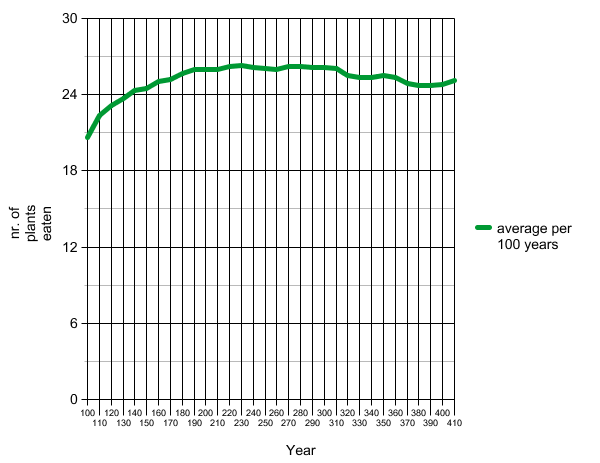
\includegraphics[width=10cm]{graph.png}\\
Crossover probability plays an important role in evolution, from the simulations we notice a difference between
between evolutions. The lower is the crossover probability, the worse an eater is evolving. This we can see on
the second graph, which represents the average plants eaten by an eater in 5 one hudred years average.\\
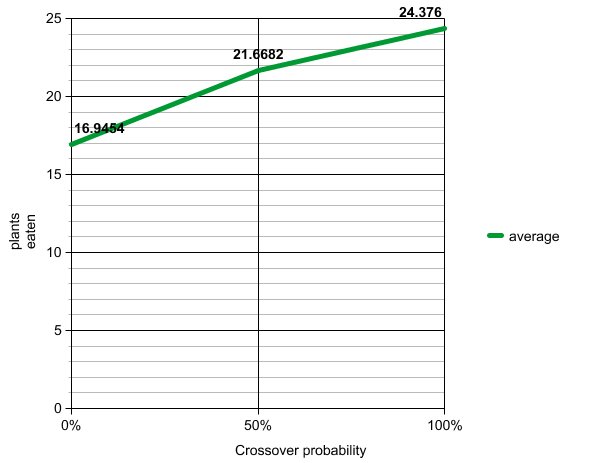
\includegraphics[width=10cm]{graph4.png}\\

\section*{Exercise 5}


\end{document}
